\documentclass[main]{subfiles}
\begin{document}

%@@@@@@@@@@@@@@@@@@@@@@@@@@@@@@
% Main Topics: vertices, extreme points and basic feasible solutions
% Linear optimization and extreme points I: 25.09.2017
% author: Vanessa Leite

\section{Linear Optimization and Extreme Points I}
Geometry can be misleading. We try to get some intuitions from geometry but
what we want to do is came up with the algebra.

Consider $\displaystyle \max_{s.t. x \in \mathcal{P}} c^{T}x, P = \{ x \in
\mathcal{R}^{n} \mid Ax \leq b \}, A \in \mathbb{Q}^{m \times n}, b \in
\mathbb{Q}^{m}, c \in \mathbb{Q}^{n}$

From linear algebra we know:\\
$A \in \mathbb{Q}^{m \times n}$\\
$n = dim(Ker(A)) + dim(Im(A))$, where $Ker(A)$ is the kernel space and $Im(A)$
is the image space.\\
$Ker(A) = \{ x \in \mathbb{R}^{n} \mid Ax = 0 \}$ \\
$Im(A) = \{ x \in \mathbb{R}^{n} \mid x^{T} = y^{T}A,\ \text{for some}\ y \in
\mathbb{R}^{n} \}$ \\
$Ker(A) \perp Im(A)$ (kernel space is orthogonal/perpendicular to image space).

$\forall z \in Im(A)$ and $\forall x \in Ker(A)$ (where z and x are vectors),
$z^{T}x = y^{T}Ax = 0$ (the dot product is zero).

\todo[inline]{definition of vector space}

\subparagraph{Definition: Let $P = \{ x \in \mathbb{R}^{n} \mid Ax \leq b \}$ be a polyhedron.}
\begin{enumerate}
\item $x \in P$ is an extreme point if there is no representation of the form
$x = \lambda y + (1- \lambda)z$ for $y, z \in P$, $y \neq z$ and $\lambda
(0,1)$.
\item $x \in P$ is an vertex if there exists $c \in \mathbb{R}^{n}$ such that
$c^{T}x > c^{T} y$, $\forall y \in P\setminus\{x\}$
\item For a point $x \in \mathbb{R}^{n}$, the index set has tight constraints:
$I(x) = \{i \in \{1, ..., m\} \mid A_{i \cdot}x = b_{i}\}$

\begin{figure}
  \label{fig:indexset}
  \centering
    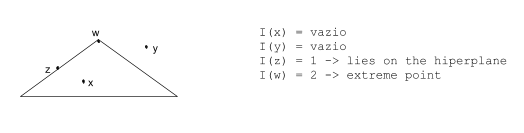
\includegraphics[width=0.8\textwidth]{imgs/indexset.png}
\end{figure}

\item $x$ is a basic solution if $dim(\{A_{i\cdot} \mid i \in I(x)\} = n$,
i.e., the vectors are linearly independent. For a basic feaseble solution,
$x \in P$.
\end{enumerate}

\subparagraph{Theorem: let $P=\{x \in \mathbb{R}^{n} \mid Ax \leq b \} \neq \emptyset$. Let
$x^{*} \in P$. The following statements are equivalent:}
\begin{enumerate}
\item $x^{*}$ is a vertex
\item $x^{*}$ is an extreme point
\item $x^{*}$ is a basic feasible solution
\end{enumerate}

\subparagraph{Proof (1 $\rightarrow$ 2):} Take a vertex $x^{*}$. That means that exist some
vector $c \in \mathbb{R}^{n}$ such that $c^{T}x^{*} > c^{T}x$, $\forall x \in
P\setminus\{x^{*}\}$. Suppose $x^{*}$ is not an extreme point.
$\exists y, z \in P$, $y \neq z$ and $\lambda \in (0,1)$ such that
$x^{*} = \lambda y + (1 - \lambda) z$

\begin{gather*}
c^{T}x^{*} = c^{T}(\lambda y + (1 - \lambda)z) \\
= \lambda c^{T}y + (1 - \lambda) c^{T}z \\
< \lambda c^{T}x^{*} + (1-\lambda) c^{T}x^{*} = c^{T}x^{*} \\
c^{T}x^{*} < c^{T}x^{*} \rightarrow contradiction!
\end{gather*}

\subparagraph{Proof (2 $\rightarrow$ 3) or ($\neg$3 $\rightarrow \neg$2):} Let $x^{*} \in P$ (so, it is feasible), assume $x^{*}$ is not a basic solution, i.e, $dim(\{A_{i\cdot} \mid i \in I(x^{*})\}) < n$.
Linear algebra tells us $\exists z \in \mathbb{R}^{n \setminus \{0\}}$ such that $A_{i\cdot} z = 0$, $\forall i \in I(x^{*})$.
\begin{gather*}
A_{i\cdot} x^{*} = b_{i}, \forall i \in I(x^{*}) \\
A_{i\cdot} x^{*} < b_{i}, \forall i \notin I(x^{*}) \\
\end{gather*}

Let
\begin{equation}
  \epsilon=\begin{cases}
    1, & \text{if $A_{i\cdot}z = 0, \forall i \notin I(x^{*})$}.\\
    min\{\frac{b_{i} - A_{i\cdot}x^{*}}{|A_{i\cdot}z|} \mid i \notin I(x^{*}) \text{ such that } A_{i\cdot}z \neq 0 & \text{otherwise}.
  \end{cases}
\end{equation}
Note $\epsilon > 0$.

Claim: $y^{+} = x^{*} + \epsilon z \in P$ and $y^{-} = x^{*} - \epsilon z \in P$. Result follows then, because
$x^{*} = \frac{1}{2}y^{+} + \frac{1}{2}y^{-}$.

\textbf{Proof of the claim:} wlog, $y^{+} \in P$. $\forall i \in I(x^{*}): A_{i\cdot} y^{+} = A_{i\cdot}x^{*} + \epsilon \underbrace{A_{i\cdot} z}_\text{$=0$} = b_{i}$

\begin{itemize}
\item $\forall i \notin I(x^{*})$ such that $ A_{i\cdot}z \leq 0$:
$A_{i\cdot} y^{+} = A_{i\cdot}x^{*} + \underbrace{\overbrace{\epsilon}^{\text{$>0$}} A_{i\cdot} z}_{\text{$\leq 0$ }} < b_{i}$
\item $\forall i \notin I(x^{*})$ such that $ A_{i\cdot}z > 0$:
Then $\epsilon \leq \frac{b_{i} - A_{i\cdot}x^{+}}{A_{i\cdot}z}$ and hence, $A_{i\cdot}y^{+} = A_{i\cdot}x^{*} + \epsilon A_{i\cdot}z$
$\leq A_{i\cdot}x^{*} + \frac{b_{i} - A_{i\cdot} x^{*}}{A_{i\cdot}z} A_{i\cdot} z = b_{i}$
\end{itemize}

\todo[inline]{do the same proof for $y^{-}$}

\subparagraph{Proof (3 $\rightarrow$ 1):} $x^{*} \in P$ is a basic feasible solution. $dim(\{A_{i\cdot} \mid i \in I(x^{*})\}) = n$

By linear algebra: $\{z \in \mathbb{R}^{n} \mid A_{i\cdot}z = 0, \forall i \in I(x^{*})\} = \{0\}$ (*) \\
Define $c^{T} = \sum_{i \in I(x^{*})}^{} A_{i\cdot} \in \mathbb{R}^{n}$ \\

$c^{T}x^{*} =  \sum_{i \in I(x^{*})}^{} A_{i\cdot}x^{*} = \sum_{i \in I(x^{*})}^{} b_{i} \underbrace{\geq}_{\forall x \in P} \sum_{i \in I(x^{*})}^{} A_{i\cdot}x = c^{T}x$ 

When is $c^{T}x^{*} = c^{T}x$? $A_{i\cdot}x = A_{i\cdot}x^{*}$, $\forall i \in I(x^{*})$
$A_{i\cdot}(x - x^{*}) = 0$, $\forall i \in I(x^{*}) \rightarrow$ (*) $x = x^{*}$

\subparagraph{Corollary: The number of vertices (extreme points or basic feasible solutions) in a Polyhedron $P$ is finite.}
\textbf{Proof:} $A \in Q^{mxn}$. The number of basic feasible solution is smaller than $m^{n}$, and it is a finite number. \\

Why are extreme points interesting for linear optimization? Consider $min 3x_{1} + 5x_{2}$

\[ 
P = \left \{
  x \in \mathbb{R}^{2} \mid
  \begin{tabular}{c}
  $2x_{1} + x_{2} \geq 3$ \\
  $2x_{1} + 2x_{2} \geq 5$ \\
  $x_{1} + 4x_{2} \geq 4$ \\
  $x_{1}, x_{2} \geq 0$ 
  \end{tabular}
\right \}
\]




\end{document}
